\section{Results}\label{results}
This section shows the main findings of the Austrian case study. As described above, results for the four scenarios Electrification (Elec), Green Gases (GG), Decentralized Green Gases and Green Methane (GM) are presented. It is structured in three parts. First, Sections \ref{res_grid2030} and \ref{res_grid2040} present the Austrian gas grid in 2030 and 2040, respectively. Section \ref{res_grid_charges} focuses on the grid costs and elaborates on the grid charges for end customers in 2040, with the quantitative results for grid length, operating, and investment costs being presented for both target years in detail.

\subsection{Austrian gas grid in 2030}\label{res_grid2030}
The Austrian gas grid in 2030 is shown in Figure \ref{fig_grid_2030}. It is the same in all four scenarios and is very similar to the initial grid in 2025, only slightly smaller. 

\begin{figure}[h]
	\centering
	\includegraphics[width=1\linewidth]{figures/results/gas_grid_2030_all_scenarios_cleaned.pdf}
	\caption{Austrian gas grid in 2030 at the transmission (blue), high-pressure (red) and mid-pressure (green) pressure levels in all four scenarios.}
	\label{fig_grid_2030}
\end{figure}

The main reason for the slight reduction of the grid length is the use of redundancies and duplicate structures in the grid as a result of declining gas demand. Table \ref{tab_compare_initial_2030} shows the reduction in the grid length at the high-pressure and mid-pressure levels in the four scenarios. 

\begin{table}[h]
	\centering
	\setlength{\extrarowheight}{.5em}
	\resizebox{0.9\textwidth}{!}{
		\begin{tabular}{lccccc}
			\toprule
			& 2025 & \multicolumn{4}{c}{2030}\\\cmidrule(lr){2-2}\cmidrule(lr){3-6}
			Pressure level & Initial grid & Elec & GG & DGG & GM\\\cmidrule(lr){1-2}\cmidrule(lr){3-6}
			\multirow{2}{*}{High-pressure} & \multirow{2}{*}{\SI{1449}{km}} & \SI{-172}{km}  & \SI{-142}{km} & \SI{-142}{km}  & \SI{-131}{km}\\
			&  & (\SI{-11.9}{\%}) & (\SI{-9.8}{\%}) & (\SI{-9.8}{\%}) & (\SI{-9.0}{\%})\\\hdashline
			\multirow{2}{*}{Mid-pressure} & \multirow{2}{*}{\SI{3218}{km}} & \SI{-283}{km}  & \SI{-200}{km} & \SI{-186}{km}  & \SI{-208}{km}\\
			& & (\SI{-8.8}{\%}) & (\SI{-6.2}{\%}) & (\SI{-5.8}{\%}) & (\SI{-6.5}{\%})\\
			\bottomrule
	\end{tabular}}
	\caption{Absolute and relative reduction in the length of the gas grid at the high-pressure and mid-pressure levels by 2030 compared to the initial grid in 2025. Abbreviations: Electrification (Elec), Green Gases (GG), Decentralized Green Gases (DGG), Green Methane (GM).}
	\label{tab_compare_initial_2030}
\end{table}

The reduction in the grid length at the high-pressure level varies between \SI{-131}{km} and \SI{-172}{km} in the GM and Elec scenarios respectively. The reduction in the grid length at the mid-pressure level varies between \SI{-186}{km} and \SI{-283}{km} in the DGG and Elec scenarios, respectively. Removing redundant gas pipelines reduces the operating costs of the grid.\footnote{In reality, these gas pipelines, especially at the transmission and high-pressure levels, can form the core of a hydrogen grid. For further details, see for example, the plans for the Austrian hydrogen grid by 2030 published by the Austrian gas grid operator \cite{aggm_agid}.} The operating costs of the gas grid, which are mainly fixed pipeline costs, decrease compared to the initial grid in 2025 and are around \SI{110}{MEUR} in all four scenarios in 2030. By 2030, virtually no gas pipelines are decommissioned due to aging or because the pipeline is no longer used to transport gas, while it is important to note that energy costs for the compressor are not included in all four scenarios. In total, those investments vary by 2030 between \SI{15}{MEUR} and \SI{18}{MEUR} in the Elec and GM scenarios, respectively, with its being of note that the rather young Austrian grid age also leads to very low replacement investments into the gas grid. Note that in the model presented in this paper, replacement investment is necessary when a pipeline reaches its technical lifetime of \SI{75}{years}. At this point, the model decides whether to invest in replacing the pipeline or to decommission it age-related. 

\subsection{Austrian gas grid in 2040}\label{res_grid2040}
The Austrian gas grid in 2040 differs significantly between the four scenarios, within which four different gas grids emerge. These four grids are mainly determined by the assumptions of the underlying scenarios. Figures \ref{fig_grid_2040_small} (Elec scenario) and \ref{fig_grid_2040_large} (GM scenario) show the smallest and largest gas grids in terms of grid length. 

\begin{figure}[h]
	\centering
	\includegraphics[width=1\linewidth]{figures/results/gas_grid_2040_elec.pdf}
	\caption{Austria's smallest gas grid by 2040 in the scenario Electrification (Elec). Colors: transmission (blue), high-pressure (red) and mid-pressure (green).}
	\label{fig_grid_2040_small}
\end{figure}

The smallest grid is in the Elec scenario and the largest in the GM scenario. They lie between the two extreme grids in terms of size. Table \ref{tab_compare_initial_2040} quantifies the size of the gas grids in 2040 in all the four scenarios by comparing the absolute length of the grids, where in absolute numbers, the reduction of grid length at the mid-pressure level is more significant than at the high-pressure level, as well as the absolute and relative reduction of grid lengths compared to the initial grid in 2025. In particular, the reduction in the grid length at the mid-pressure level is equally greatest in the two scenarios Elec and GG with \SI{-1316}{km} (\SI{-40.9}{\%} compared to the initial grid in 2025). The smallest reduction in length at the mid-pressure level among the four scenarios is with \SI{-811}{km} (\SI{-25.2}{\%} compared to the initial grid in 2025) in the DGG scenario. 

\begin{figure}[h]
	\centering
	\includegraphics[width=1\linewidth]{figures/results/gas_grid_2040_gm.pdf}
	\caption{Austria's largest gas grid by 2040 in the scenario Green Methane (GM). Colors: transmission (blue), high-pressure (red) and mid-pressure (green).}
	\label{fig_grid_2040_large}
\end{figure}

The main reason here for the relatively small reduction in the mid-pressure grid length is the significant decentralized generation and injection of domestic renewable gas. 

\begin{table}[h!]
	\centering
	\setlength{\extrarowheight}{.5em}
	\resizebox{1\textwidth}{!}{
		\begin{tabular}{llrrrr}
			\toprule
			& & \multicolumn{4}{c}{2040}\\\cmidrule(lr){3-6}
			Pressure level & Indicator & \multicolumn{1}{c}{Elec} & \multicolumn{1}{c}{GG} & \multicolumn{1}{c}{DGG} & \multicolumn{1}{c}{GM}\\\cmidrule(lr){1-2}\cmidrule(lr){3-6}
			\multirow{3}{*}{High-pressure} & Abs. grid length in 2040& \SI{964}{km}  & \SI{965}{km} & \SI{974}{km}  & \SI{1105}{km}\\
			 & Abs. reduction to 2025 & \SI{-485}{km}  & \SI{-484}{km} & \SI{-475}{km}  & \SI{-344}{km}\\
			 & Rel. reduction to 2025 & \SI{-33.5}{\%}& \SI{-33.4}{\%}& \SI{-32.8}{\%}&\SI{-23.7}{\%}\\\hdashline
 			\multirow{3}{*}{Mid-pressure} & Abs. grid length in 2040& \SI{1902}{km}  & \SI{1902}{km} & \SI{2407}{km}  & \SI{2331}{km}\\
			 & Abs. reduction to 2025 & \SI{-1316}{km}  & \SI{-1316}{km} & \SI{-811}{km}  & \SI{-887}{km}\\
			 & Rel. reduction to 2025 & \SI{-40.9}{\%}& \SI{-40.9}{\%}& \SI{-25.2}{\%}&\SI{-27.6}{\%}\\
			\bottomrule
	\end{tabular}}
	\caption{Absolute length of the grids 2040 in the four scenarios as well as the absolute and relative reduction of grid lengths compared to the initial grid in 2025 at the high-pressure and mid-pressure levels. Abbreviations: Electrification (Elec), Green Gases (GG), Decentralized Green Gases (DGG), Green Methane (GM).}
	\label{tab_compare_initial_2040}
\end{table}

The domestic injection leads to an increased use of mid-pressure pipelines. Figure \ref{fig_reduction_waterfall} shows the grid length in the two extreme scenarios Elec (top) and GM (bottom) at high-pressure (left) and mid-pressure (right) levels. It highlights the reduction in grid length by 2030 and 2040. The grid length in 2025 is shown on the far left and in 2040 on the far right. 

\begin{figure}[h]
	\begin{subfigure}[c]{0.5\textwidth}
		\centering
		\includegraphics[width=1\linewidth]{figures/results/waterfall/waterfall_elec_high.pdf}
		\vspace{-0.6cm}
		\subcaption{Elec | High-pressure}
		\label{Fig:a}
	\end{subfigure}
	\begin{subfigure}[c]{0.5\textwidth}
		\centering
		\includegraphics[width=1\linewidth]{figures/results/waterfall/waterfall_elec_mid.pdf}
		\vspace{-0.6cm}
		\subcaption{Elec  | Mid-pressure}
		\label{Fig:b}
	\end{subfigure}
	\newline
	\newline
	\newline
	\begin{subfigure}[c]{0.5\textwidth}
		\centering
		\includegraphics[width=1\linewidth]{figures/results/waterfall/waterfall_gm_high.pdf}
		\vspace{-0.6cm}
		\subcaption{GM | High-pressure}
		\label{Fig:c}
	\end{subfigure}
	\begin{subfigure}[c]{0.5\textwidth}
		\centering
		\includegraphics[width=1\linewidth]{figures/results/waterfall/waterfall_gm_mid.pdf}
		\vspace{-0.6cm}
		\subcaption{GM | Mid-pressure}
		\label{Fig:d}
	\end{subfigure}
	\caption{Comparison of the Austrian gas grid in 2025 and 2040 in the extreme scenarios Electrification (Elec) and Green Methane (GM) at high-pressure and mid-pressure levels. In the Elec and GM scenarios, the smallest and the largest gas grids are obtained in terms of the size of the grids.}
	\label{fig_reduction_waterfall}
\end{figure}

The operating costs of the gas grid decrease compared to 2025. They vary between \SI{87.5}{MEUR} and \SI{93.0}{MEUR} in the Elec and GM scenarios, respectively. With the remaining costs being accounted by the high-pressure and mid-pressure level, \SI{50.0}{MEUR} (the same in all four scenarios) are accounted for the transmission level. Figure \ref{fig_grid_repl_inv} shows the total replacement investments in the gas grid in the four scenarios. It includes the replacement investments in 2030 mentioned in Section \ref{res_grid2030} above. The lowest total replacement investments are in the scenarios GG and Elec with \SI{143.0}{MEUR} and \SI{146.0}{MEUR} respectively. The highest replacement investments are in the GM scenario with \SI{185.0}{MEUR}. 

\begin{figure}[h]
	\centering
	\includegraphics[width=0.8\linewidth]{figures/results/total_replacement_inv/replace_inv_2040.pdf}
	\caption{Total replacement investments in the Austrian gas grid until 2040 in the four scenarios.}
	\label{fig_grid_repl_inv}
\end{figure}

The off-grid solution is not used in the four scenarios, with the model not choosing the off-grid solution due to its high costs, except in very few cases, with this also being true when meager amounts of gas are transported through gas pipelines. The economic trade-off between a scarcely utilized gas pipeline and the off-grid solution is illustrated in Figure \ref{line_and_point} in \ref{app_off_grid}.

\subsection{Grid charges for customers in 2040}\label{res_grid_charges}
This section presents an analysis of the cost-effectiveness of the gas grid in four different scenarios. In average grid costs serving as a basis for estimating grid charges for customers in 2040, the average grid costs are calculated by dividing the total annual grid costs by the gas demand supplied. It should be noted that determining grid charges based on minimizing system costs must be viewed with caution, although regulatory mechanisms often rely on approaches that aim to minimize system costs, as a grid charge regulation process must also take other considerations into account. Therefore, it is important to consider and interpret the following results from this perspective. In particular, the different grid costs provide a different perspective on comparing the four scenarios.\vspace{0.3cm}

Noting that the horizontal axis is the renewable gas demand supplied by the grid in TWh, Figure \ref{fig_grid_charges} shows the (average) grid costs in 2040 in the four different scenarios. The Elec scenario, as it has the lowest gas demand of the four scenarios, is therefore on the far left. At the same time, the GM scenario, which has the highest gas demand among the scenarios, is on the far right. 

\begin{figure}[h]
	\centering
	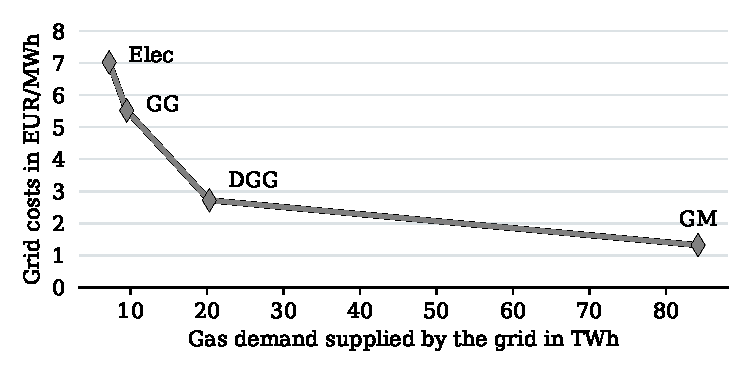
\includegraphics[width=1\linewidth]{figures/results/grid_charges/grid_charges.pdf}
	\caption{Grid costs in the four scenarios Electrification (Elec), Green Gases (GG), Decentralized Green Gases (DGG) and Green Methane (GM).}
	\label{fig_grid_charges}
\end{figure}

It is shown that the grid costs are the highest in the Elec scenario with \SI{7.0}{EUR \per MWh} and the lowest in the GM scenario with \SI{1.3}{EUR \per MWh}. The grid costs and its components of operating costs at the different pressure levels and gas demand supplied are summarized in Table \ref{tab_components_grid_costs}. Note that the transmission operating costs accounted for customers in these scenarios are zero, as the three scenarios Elec, GG and DGG assume a separation between the transmission and distribution grids (i.e., high and medium pressure levels). Consequently, it is assumed that customers requesting gas transport through Austria at the transmission level bear these costs. A comparison of the average grid costs with the current grid charges in Austria shows that these are increasing significantly in three of the four scenarios. The current grid charges at the mid-pressure level in Austria are around \SI{1.7}{EUR \per MWh} \cite{econtrol_gas_charges}.

\begin{table}[h!]
	\centering
	\setlength{\extrarowheight}{.5em}
	\resizebox{0.85\textwidth}{!}{
		\begin{tabular}{lrrrr}
			\toprule
			& \multicolumn{4}{c}{2040}\\\cmidrule(lr){2-5}
			Components for calculating grid costs & Elec & GG & DGG & GM\\\hline
			Transmission operating costs in MEUR & 0 & 0 &0  & \SI{50}{}\\
			Distribution operating costs in MEUR & \SI{37.5}{} & \SI{39.3}{} & \SI{40.2}{} & \SI{43.0}{}\\
			Capital costs per year in MEUR & \SI{13.0}{} & \SI{13.1}{} & \SI{15.0}{} & \SI{18.3}{}\\
			Gas demand supplied in TWh & \SI{7.2}{} & \SI{9.5}{} & \SI{20.3}{} & \SI{84.2}{}\\\hline
			Grid costs in EUR/MWh & \SI{7.0}{} & \SI{5.5}{} & \SI{2.7}{} & \SI{1.3}{}\\
			\bottomrule
	\end{tabular}}
	\caption{Average grid costs and their components of operating costs and capital costs. The distribution operating costs encompass the high-pressure and mid-pressure levels. Separation between the transmission and distribution grids result in accounting no transmission operating costs for the customers.}
	\label{tab_components_grid_costs}
\end{table}

 Only in the GM scenario, where the supply depends on massive renewable imports, do the grid costs remain around or slightly below this value. In the results of the other three scenarios, the increase in grid costs is driven by the high operating costs of the distribution grid with comparatively low demand volumes and capital costs. Necessary due to the aging of the (otherwise already fully depreciated) existing grid, the (annual) capital costs in 2040 result essentially from the replacement investments made by then. As mentioned, a technical lifetime of the pipelines of \SI{75}{years} is assumed. A possible window for reducing grid costs opens, as a more extended operation of pipelines (e.g., technical lifetime between 90 and \SI{100}{years}) could reduce the share of capital costs in the grid costs; in extreme cases even go toward zero. Such a measure of a longer operating life of pipelines is certainly considered in practice, especially against the background of declining transport volumes. This is because transport volumes determine the operating pressure levels, which determine the pipelines' wear and tear. While replacement investments due to aging could be saved, lowering the operating pressure levels compared to today's could extend the technical lifetime\footnote{In addition, lowering the operating pressure levels also affects and supports domestic renewable gas generation. On the one hand, generation plants require less energy to compress their gas, and on the other hand, their connection costs are reduced, as the costs are highly dependent on the pressure levels in the grid. For more information from the field, see \cite{biogas_einspeisung}.}. Figure \ref{fig_grid_charges_no_capex} shows the impact on the grid costs if an extension of the pipelines' technical lifetime to \SI{90}{}-\SI{100}{years} is taken into account. With grid costs consequently going down in all the four scenarios, the lifetime extension leads to no replacement investments and the current pipelines can remain in operation. The highest reduction in grid costs is with \SI{-1.8}{EUR/MWh} in the Elec scenario. The latter is the one with initially the highest grid costs. The smallest reduction in grid costs is with \SI{-0.2}{EUR/MWh} in the GM scenario.

\begin{figure}[h]
	\centering
	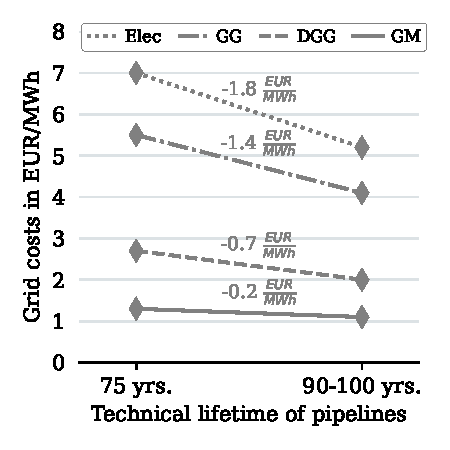
\includegraphics[width=0.6\linewidth]{figures/results/grid_charges_development/cleaned_grid_charges.pdf}
	\caption{Comparison of grid costs in 2040 for a technical lifetime of pipelines of \SI{75}{years} (left) and 90-\SI{100}{years} (right).}
	\label{fig_grid_charges_no_capex}
\end{figure}
